\begin{problem}{1.6}{problem1_6}

For the DC motor modeled by
\begin{equation}
	\begin{aligned}
		J\frac{d\omega}{dt} & = k_m i - T_L,          \\
		L\frac{di}{dt}      & = -iR - k_b \omega + u,
	\end{aligned}
	\label{eq:dcmotor}
\end{equation}
where \( J \) is the moment of inertia, \( i \) is the armature current, \( L \) and \( R \) are the armature inductance and resistance respectively, \( \omega \) is the motor angular speed, \( k_b \) is a constant of back electromotive force, \( k_m \) is a motor torque constant, \( T_L \) is an unknown load torque which is bounded and has a bounded derivative, and \( u \) is a control function defined by the armature voltage.

Design a sliding mode control \( u \), steering the angular speed \( \omega \) to zero assuming both \( i \) and \( \omega \) are measurable and all parameters are known. Simulate the control system with the following parameters:
\[
	\begin{aligned}
		R         & = 1\,\Omega,                        \\
		L         & = 0.5\,\text{H},                    \\
		k_m       & = 5 \times 10^{-2}\,\text{Nm/A},    \\
		k_b       & = k_m,                              \\
		J         & = 10^{-3}\,\text{Nms}^2/\text{rad}, \\
		T_L       & = 0.1 \sin(t)\,\text{Nm},           \\
		\omega(0) & = 1\,\text{rad/s},                  \\
		i(0)      & = 0.
	\end{aligned}
\]

Plot the time histories of the sliding variable, the control function \( u \), the current \( i \), and the angular speed \( \omega \).

\end{problem}

\begin{solution}{}{solution1_6}
	The system \eqref{eq:dcmotor} can be represented in state-space form as:
	\[
		\begin{aligned}
			\dot{x}_1 & = \frac{k_m}{J} x_2 - \frac{T_L}{J}, \\
			\dot{x}_2 & = -\frac{k_b}{L} x_1 - \frac{R}{L} x_2 + \frac{1}{L} u,
		\end{aligned}
	\]
	where \( x_1 = \omega \) (angular speed) and \( x_2 = i \) (armature current).

	The control objective is to drive \( \omega = x_1 \to 0 \) as \( t \to \infty \). To this end, we define the sliding variable as
	\[
		\begin{aligned}
			s & = \dot{x}_1 + \lambda x_1 \\
			  & = \frac{k_m}{J} x_2 - \frac{T_L}{J} + \lambda x_1.
		\end{aligned}
	\]
	The term \( -\frac{T_L}{J} \) is considered as an unmatched disturbance, letś redefine the sliding variable as:
	\[
		s = \frac{k_m}{J} x_2 + \lambda x_1.
	\]

	On the sliding surface \( s = 0 \), the dynamics reduce to:
	\[
		x_2 = -\frac{\lambda J}{k_m} x_1.
	\]
	Substituting into the first state equation yields:
	\[
		\dot{x}_1 = -\lambda x_1 - \frac{T_L}{J}.
	\]
    Thus, the disturbance that enters in the first equation (where control is absent) will prevent the state variable from converging to zero in the sliding mode. Nevertheless, let's continue with the typical approach to see this fenomena.\\

	Consider the Lyapunov candidate:
	\[
		V = \frac{1}{2} s^2 \quad \Rightarrow \quad \dot{V} = s \dot{s}.
	\]
	Computing \( \dot{s} \), we have:
	\[
		\dot{s} = \frac{k_m}{J} \dot{x}_2 + \lambda \dot{x}_1 = \frac{k_m}{J} \left( -\frac{k_b}{L} x_1 - \frac{R}{L} x_2 + \frac{1}{L} u \right) + \lambda \left( \frac{k_m}{J} x_2 - \frac{T_L}{J} \right).
	\]
	Simplifying, we can express \( \dot{V} \) as:
	\[
		\dot{V} = s \left[ k_m \left( -\left(\frac{R}{L} + \lambda \right) x_2 - \frac{k_b}{L} x_1 + \frac{1}{L} u \right) - \lambda T_L \right].
	\]

	To enforce \( \dot{s} = -\rho\, \text{sign}(s) \), with \( \rho > 0 \), we choose the control input:
	\[
		u = (R - \lambda L) x_2 + k_b x_1 + \frac{L}{k_m} v,
	\]
	where \( v = -\rho\, \text{sign}(s) \).

	Substituting into the Lyapunov derivative:
	\[
		\dot{V} = s \left[ -\lambda T_L + v \right].
	\]
	To ensure \( \dot{V} < 0 \), we bound the disturbance: \( |T_L| \leq 0.1 \). Then:
	\[
		\dot{V} \leq \lambda \cdot 0.1 |s| + s v = \lambda \cdot 0.1 |s| - \rho |s| = -|s|(\rho - 0.1\lambda).
	\]
	Hence, choosing \( \lambda = 1 \) and \( \rho = 0.2 \), the condition \( \dot{V} < 0 \) is guaranteed.\\

	Simulation results with this control strategy are presented below.

    \begin{figure}[H]
        \centering
        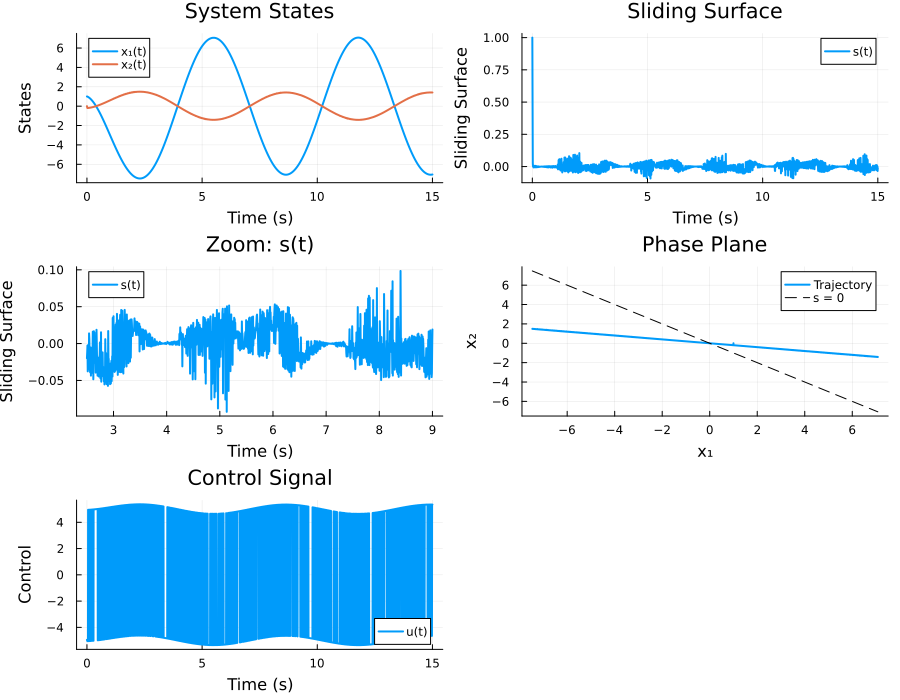
\includegraphics[width=1\textwidth]{img/problem1_6.png}
        \caption{Simulation results for the sliding mode control system.}
        \label{fig:problem1_6}
    \end{figure}
    The simulation shows that the system converges to the sliding mode, but the disturbance \( T_L \) prevents the $x_1 = \omega$ state variable from converging asymptotically to zero.
\end{solution}
